\documentclass{beamer}
\usetheme{metropolis}           % Use metropolis theme
\usepackage[outputdir=./.latex-out]{minted} % TODO slet hvis du ikke bruger minted
\newcommand{\tex}[1] {
  \mintinline{latex}{#1}
}
\usepackage{listings}
\title{\LaTeX Webinar}
\date{\today}
\author{Benjamin Rotendahl}
\institute{Study Now}
\begin{document}
\maketitle
\section{Velkommen og plan for idag}
 \begin{frame}{Planen for idag}
   Formålet med dette webinar er at skabe give en kort introduktion til LaTeX,
   så i har den nødvendige baggrundsviden for at kaste jer ud i det.
   Webinaret dækker:
   \begin{itemize}
     \item Hvordan man kompilerer \LaTeX og går fra kildekode til PDF \pause
     \item Syntaksen og gængse udtryk \pause
     \item Håndtering af matematik \pause
     \item Grafer, tabeller og kode
   \end{itemize}
 \end{frame}

 \begin{frame}{Fra kode til PDF}
   \LaTeX{} adskiller sig fra programmer som word, google docs, osv. ved ikke at
   være en så såkaldt \emph{WYSIWYG}\footnote{What you see is what you get} editor.
   \pause
   I stedet for at trykke på en knap for at lave noget kursiv skriver man:
   \centering\tex{\emph{det vigtige}}
 \end{frame}

 \begin{frame}{Fra kode til PDF}
   \begin{figure}[h]
     \centering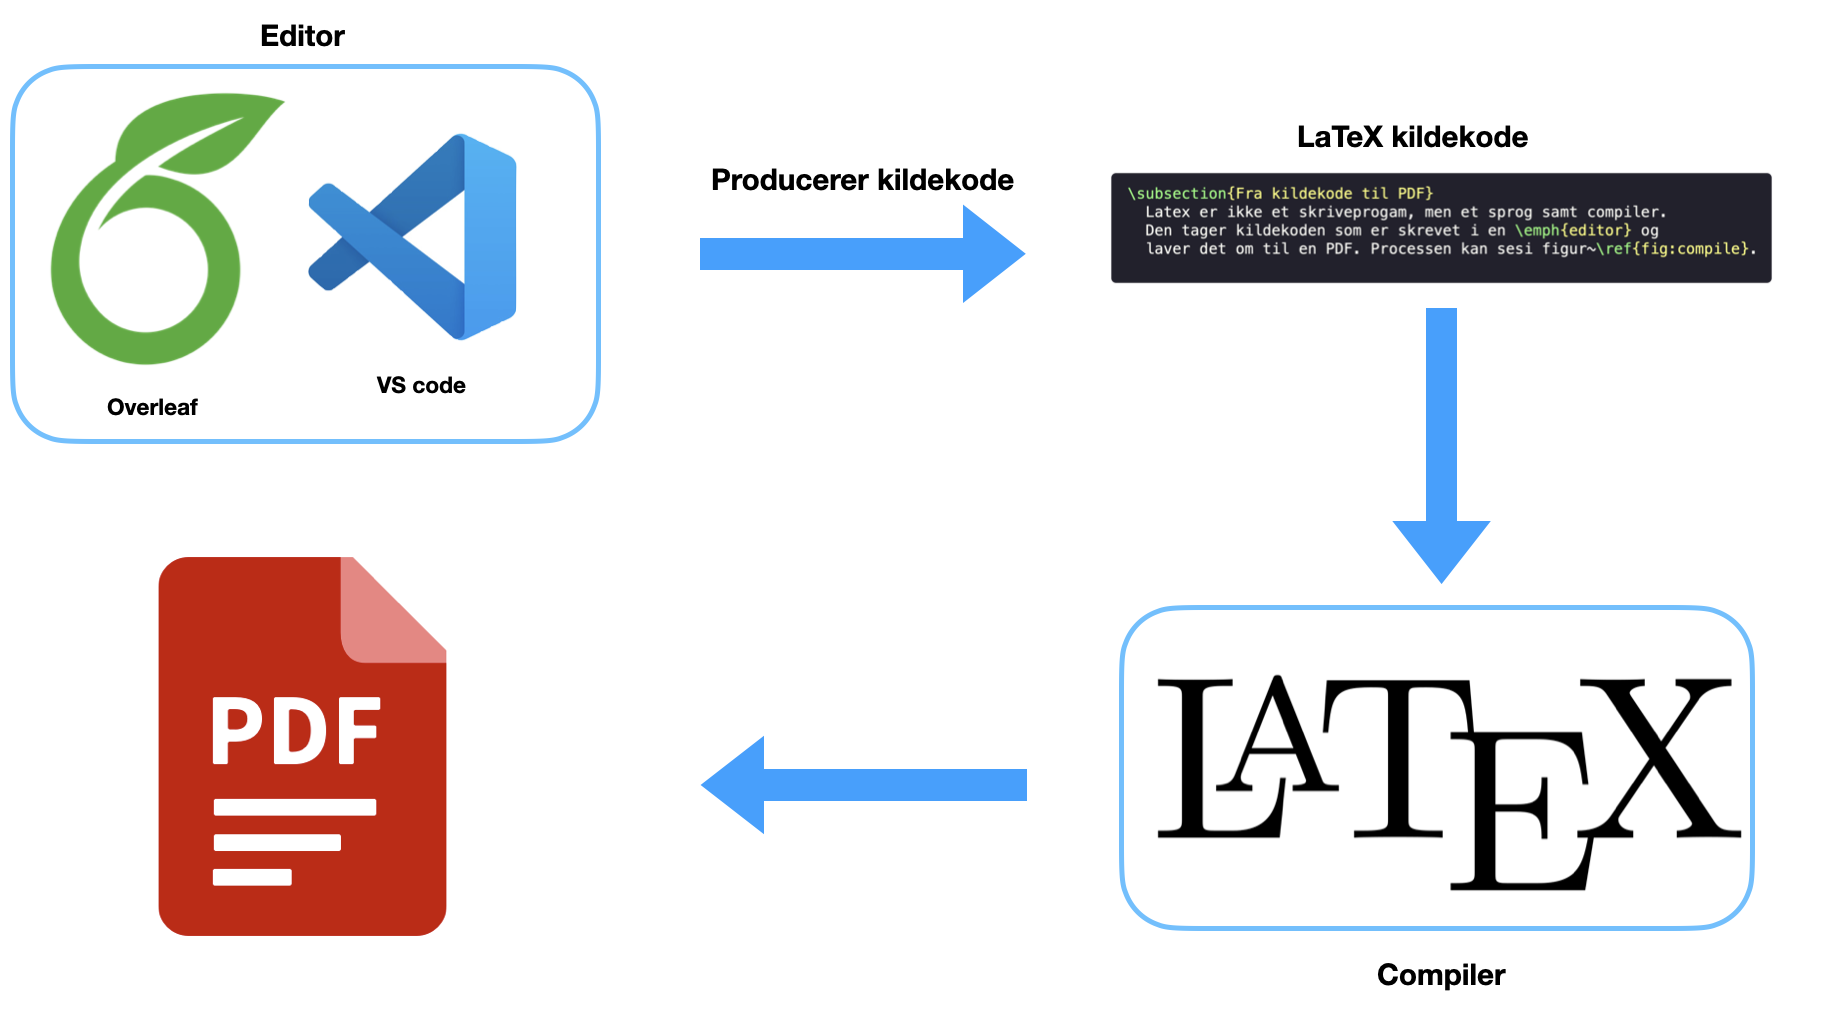
\includegraphics[width=0.9\textwidth]{../assets/compile.png}
     \caption{Hvordan man kommer fra kildekode til pdf}\label{fig:compile}
   \end{figure}
 \end{frame}

 \begin{frame}{\LaTeX styrker}
   Den primære styrke er at det er nemt at skrive matematik:
   \begin{flalign}
     f(x, y)                       & = 3x^2y + y^2 +  \left ( \frac{2^3}{6} \right )^2 \\
     \frac{\partial f}{\partial x} & = 6xy                                             \\
     \frac{\partial f}{\partial y} & = 3x^2 + 2y                                       \\
     \mathbf{z}                    & =  \begin{pmatrix}
                                            1 & 2 & 3 \\
                                            4 & 5 & 6 \\
                                            7 & 8 & 9
                                          \end{pmatrix}
   \end{flalign}
 \end{frame}

\end{document}